\include{settings}

\begin{document}	% начало документа

% Титульная страница
\begin{titlepage}	% начало титульной страницы

	\begin{center}		% выравнивание по центру

		\large Санкт-Петербургский политехнический университет Петра Великого\\
		\large Физико-механический институт \\
		\large Высшая школа прикладной математики и вычислительной физики\\[3cm]
		% название института, затем отступ 6см
		\large Направление подготовки\\
		\large "01.03.02. Прикладная математика и информатика"\\[3cm]
		\huge Дисциплина "Численные методы"\\[0.5cm] % название работы, затем отступ 0,5см
		\large Отчет по лабораторной работе №4\\[0.1cm]
		\large "Решение алгебраической проблемы собственных значений итерационными методами. Степенной метод для поиска второго максимального по модулю собственного значения и соответствующего собственного вектора"\\[5cm]

	\end{center}


	\begin{flushright} % выравнивание по правому краю
		\begin{minipage}{0.25\textwidth} % врезка в половину ширины текста
			\begin{flushleft} % выровнять её содержимое по левому краю

				\large\textbf{Работу выполнил:}\\
				\large Иванова А.С.\\
				\large {Группа:} 5030102/00002\\
				
				\large \textbf{Преподаватель:}\\
				\large Курц В.В.

			\end{flushleft}
		\end{minipage}
	\end{flushright}
	
	\vfill % заполнить всё доступное ниже пространство

	\begin{center}
	\large Санкт-Петербург\\
	\large \the\year % вывести дату
	\end{center} % закончить выравнивание по центру

\end{titlepage} % конец титульной страницы

\vfill % заполнить всё доступное ниже пространство


\include{ToC}

\section{Формулировка задачи}

Решить СЛАУ, используя метод вращений. Проверить вычислительную ошибку (сравнивая с точным решением) для матриц с разными числами 
обусловленности.

Уравнение в матричном виде 

\begin{math}
	Ax=b
\end{math},
где A - матрица системы, b - столбец свободных членов, x - вектор-столбец неизвестных (который нужно найти)

\section{Алгоритм метода и условия его применимости}

Условия применимости: 

Матрица системы должны быть невырожденной (определитель матрицы не равен 0).


Пусть \begin{math}
	c_{12}
\end{math} и
 \begin{math}
 	s_{12}
 \end{math} - некоторые отличные от нуля числа.

Новое 1-­е уравнение ­ линейная комбинация 1-­го и 2-го уравнений с коэффициентами 
\begin{math}
	c_{12}
\end{math} и
\begin{math}
	s_{12}
\end{math}  .

Новое 2-­е уравнение ­ линейная комбинация 1-­го и 2-го уравнений с коэффициентами 
\begin{math}
	-s_{12}
\end{math} и
\begin{math}
	c_{12}
\end{math}  .

\begin{math}
	(c_{12}a_{11}+s_{12}a_{21})x_{1}+...+(c_{12}a_{1n}+s_{12}a_{2n})x_{n}=c_{12}b_{1}+s_{12}b_{2}
\end{math}

\begin{math}
	(-s_{12}a_{11}+c_{12}a_{21})x_{1}+...+(-s_{12}a_{1n}+c_{12}a_{2n})x_{n}=-s_{12}b_{1}+c_{12}b_{2}
\end{math}

Условия на 
\begin{math}
	c_{12}
\end{math} и
\begin{math}
	s_{12}
\end{math}  

\begin{math}
	(-s_{12}a_{11}+c_{12}a_{21})=0 
\end{math}
,
\begin{math}
	c_{12}^{2}+s_{12}^{2}=1
\end{math}
 
 Тогда
 
 \begin{math}
 	c_{12}=\frac{a_{11}}{\sqrt{a_{11}^{2}+a_{21}^{2}}}
 \end{math},
\begin{math}
	s_{12}=\frac{a_{21}}{\sqrt{a_{11}^{2}+a_{21}^{2}}}
\end{math}.

Данное преобразование эквивалентно умножению A и b на 
\begin{math}
	T_{12}
\end{math} слева

\begin{equation*}
	T_{12} = \left(
	\begin{array}{ccccc}
		c_{12} & s_{12} & 0 & \ldots & 0\\
		-s_{12} & c_{12} & 0 & \ldots & 0\\
		0 & 0 & 1 & \ldots & 0\\
		\vdots & \vdots & \vdots & \ddots & \vdots\\
		0 & 0 & 0 & \ldots & 1
	\end{array}
	\right)
\end{equation*}


\begin{math}
	T_{12}
\end{math} 
- матрица вращения в плоскости 
\begin{math}
	O_{x_{1}x_{2}}
\end{math}
на угол 
\begin{math}
	\phi_{12}
\end{math} 
такой, что 
\begin{math}
	\cos (\phi_{12}) = c_{12}
\end{math} ,
\begin{math}
	\sin (\phi_{12}) = s_{12}
\end{math} 
 
 Исключим 
 \begin{math}
 	x_{1}
 \end{math} 
из 3-го уравнения с помощью 
\begin{math}
	c_{13}
\end{math} и
\begin{math}
	s_{13}
\end{math} 

\begin{math}
	c_{13}=\frac{a_{11}^{(1)}}{\sqrt{(a_{11}^{(1)})^{2}+a_{31}^{2}}}
\end{math},
\begin{math}
	s_{13}=\frac{a_{31}}{\sqrt{(a_{11}^{(1)})^{2}+a_{31}^{2}}}
\end{math}

Это эквивалентно усножению СЛАУ слева на 
\begin{math}
	T_{13}
\end{math}

\begin{equation*}
	T_{13} = \left(
	\begin{array}{ccccc}
		c_{13} & 0 & s_{13}  & \ldots & 0\\
		0 & 1 & 0 & \ldots & 0\\
		-s_{13} & 0 & c_{13} & \ldots & 0\\
		\vdots & \vdots & \vdots & \ddots & \vdots\\
		0 & 0 & 0 & \ldots & 1
	\end{array}
	\right)
\end{equation*}

После n − 1 таких преобразований

\begin{math}
	a_{11}^{(n-1)}x_{1}+a_{12}^{(n-1)}x_{2}+...+a_{1n}^{(n-1)}x_{n}=b_{1}^{(n-1)}
\end{math}

\begin{math}
	a_{22}^{(1)}x_{2}+...+a_{2n}^{(1)}x_{n}=b_{2}^{(1)}
\end{math}

...   ...   ...   ...

\begin{math}
	a_{n2}^{(1)}x_{2}+...+a_{nn}^{(1)}x_{n}=b_{n}^{(1)}
\end{math}

Второй шаг метода вращений - исключение 
\begin{math}
	x_{2}
\end{math} 
из всех уравнений, начиная с 3-го. В результате выполнения n-2 подшагов СЛАУ преобразуется к виду

\begin{math}
	a_{11}^{(n-1)}x_{1}+a_{12}^{(n-1)}x_{2}+a_{13}^{(n-1)}x_{3}+...+a_{1n}^{(n-1)}x_{n}=b_{1}^{(n-1)}
\end{math}

 \begin{math}
 	a_{22}^{(n-1)}x_{2}+a_{23}^{(n-1)}x_{3}+...+a_{2n}^{(n-1)}x_{n}=b_{2}^{(n-1)}
 \end{math}

\begin{math}
	a_{33}^{(2)}x_{3}+...+a_{3n}^{(2)}x_{n}=b_{3}^{(2)}
\end{math}
... ... ... ...

\begin{math}
	a_{n3}^{(2)}x_{3}+...+a_{nn}^{(2)}x_{n}=b_{n}^{(2)}
\end{math}
 
После завершения n-1 шага система имеет вид 

\begin{math}
	a_{11}^{(n-1)}x_{1}+a_{12}^{(n-1)}x_{2}+a_{13}^{(n-1)}x_{3}+...+a_{1n}^{(n-1)}x_{n}=b_{1}^{(n-1)}
\end{math}

\begin{math}
	a_{22}^{(n-1)}x_{2}+a_{23}^{(n-1)}x_{3}+...+a_{2n}^{(n-1)}x_{n}=b_{2}^{(n-1)}
\end{math}

\begin{math}
	a_{33}^{(n-1)}x_{3}+...+a_{3n}^{(n-1)}x_{n}=b_{3}^{(n-1)}
\end{math}

... ... ... ...

\begin{math}
	a_{n3}^{(n-1)}x_{3}+...+a_{nn}^{(n-1)}x_{n}=b_{n}^{(n-1)}
\end{math}
 
В матричной записи 
 
\begin{math}
	A^{(n-1)}x=b^{(n-1)}
\end{math}, 

где 

\begin{math}
	A^{(n-1)}=T_{n-1,n}A^{(n-2)}
\end{math},

\begin{math}
	b^{(n-1)}=T_{n-1,n}b^{(n-2)}
\end{math}

Матрица системы - верхняя треугольная, причем 

\begin{math}
	A^{(n-1)}=TA
\end{math},
где 

\begin{math}
	T=T_{n-1,n}...T_{2n}...T_{23}T_{1n}...T_{12}
\end{math} 
- матрица результирующего вращения 

Матрица T ортогональна как произведение ортогональных матриц. Обозначим 
\begin{math}
	Q=T^{-1}=T^{T}
\end{math},
получили QR-разложение матрицы A.

Обратный ход метода вращений проводится точно так же, как и для метода Гаусса.

\section{Предварительный анализ задачи}

В системе MATLAB матрицы генерируются таким образом, что определитель матрицы системы точно не равняется нулю. Следовательно система имеет единственное решение. 

\section{Проверка условий применимости метода}

В системе MATLAB матрицы генерируются таким образом, что определитель матрицы системы точно не равняется нулю. Условие выполнено.

\section{Тестовый пример с детальными расчетами для задачи малой размерности}

Решим систему уравнений

\begin{equation*}
	\begin{cases}
		x_{1}+2x_{2}+3x_{3}&=8\\
		3x_{1}+x_{2}+x_{3}&=3\\
		2x_{1}+3x_{2}+x_{3}&=8
	\end{cases}
\end{equation*}

Найдем определитель матрицы системы, чтобы убедиться, что она невырожденная 

\begin{equation*}
	\det A =
	\begin{vmatrix}
		1 & 2 & 3\\
		3 & 1 & 1\\
		2 & 3 & 1
	\end{vmatrix}
	= 17
\end{equation*}

Данная система имеет единственное решение.
 
Найдем  \begin{math}
	c_{12}
\end{math} и
\begin{math}
	s_{12}
\end{math}

\begin{math}
	-s_{12}+3c_{12}=0
\end{math}

\begin{math}
	c_{12}=\frac1{\sqrt{10}}
\end{math}

\begin{math}
	s_{12}=\frac3{\sqrt{10}}
\end{math}

Подставим эти значения в первые два уравнения системы, получим новую систему:

\begin{equation*}
	\begin{cases}
		10x_{1}+5x_{2}+6x_{3}&=17\\
		-5x_{2}-8x_{3}&=-21\\
		2x_{1}+3x_{2}+x_{3}&=5
	\end{cases}
\end{equation*}

Найдем 
\begin{math}
	c_{13}
\end{math} и
\begin{math}
	s_{13}
\end{math}

\begin{math}
	-10s_{13}+2c_{13}=0
\end{math}

\begin{math}
	c_{13}=\frac5{\sqrt{26}}
\end{math}

\begin{math}
	s_{13}=\frac1{\sqrt{26}}
\end{math}

Подставим эти значения в уравнения 1 и 3 системы, получим систему:

\begin{equation*}
	\begin{cases}
		52x_{1}+28x_{2}+31x_{3}&=90\\
		-5x_{2}-8x_{3}&=-21\\
		-10x_{2}-x_{3}&=-8
	\end{cases}
\end{equation*}

Найдем
\begin{math}
	c_{23}
\end{math} и
\begin{math}
	s_{23}
\end{math}

\begin{math}
	10s_{23}-5c_{23}=0
\end{math}

\begin{math}
	c_{23}=-\frac1{\sqrt{5}}
\end{math}

\begin{math}
	s_{12}=-\frac2{\sqrt{5}}
\end{math}

Подставим найденные значения во 2 и 3 уравнения системы и найдем результирующую систему:

\begin{equation*}
	\begin{cases}
		52x_{1}+28x_{2}+31x_{3}&=90\\
		35x_{2}-10x_{3}&=15\\
		-15x_{3}&=-30
	\end{cases}
\end{equation*}

Далее простыми алегбраическими преобразованиями находим решение системы:

\begin{equation*}
	\begin{cases}
		x_{1}&=0\\
		x_{2}&=1\\
		x_{3}&=2
	\end{cases}
\end{equation*}

Проверяем решение в MATLAB

\includegraphics[scale=0.5]{test.png}


\section{Перечень контрольных тестов для иллюстрации метода}

\subsection{Зависимость относительной погрешности от числа обусловленности}

Размерность матрицы фиксирована (15 на 15), матрица чисел обусловленности задана в MATLAB, числа обусловленности меняются в цикле от 10 до 50000. Точное решение всех систем в цикле одинаково (представляет собой столбец единиц). Ожидается, что с ростом числа обусловленности относительная погрешность будет увеличиваться

\subsection{Зависимость относительной погрешности решения от относительной погрешности возмущения}

Матрица системы, ее размерность и число обусловленности фиксированы, меняется столбец свободных членов. В первом случае число обусловленности равно 100, во втором случае число обусловленности равно 1000000000, все элементы столбца свободных членов меняются от 1 до 2 с шагом 0.001. Ожидается, что относительная погрешность решения при большем числе обусловленности будет больше.

\section{Модульная структура программы}

Функция long double** ArrayRead(FILE* file, int line, int column)

\includegraphics[scale=0.5]{block1.pdf}

Функция void RotationMethod(long double** A,long double* b)

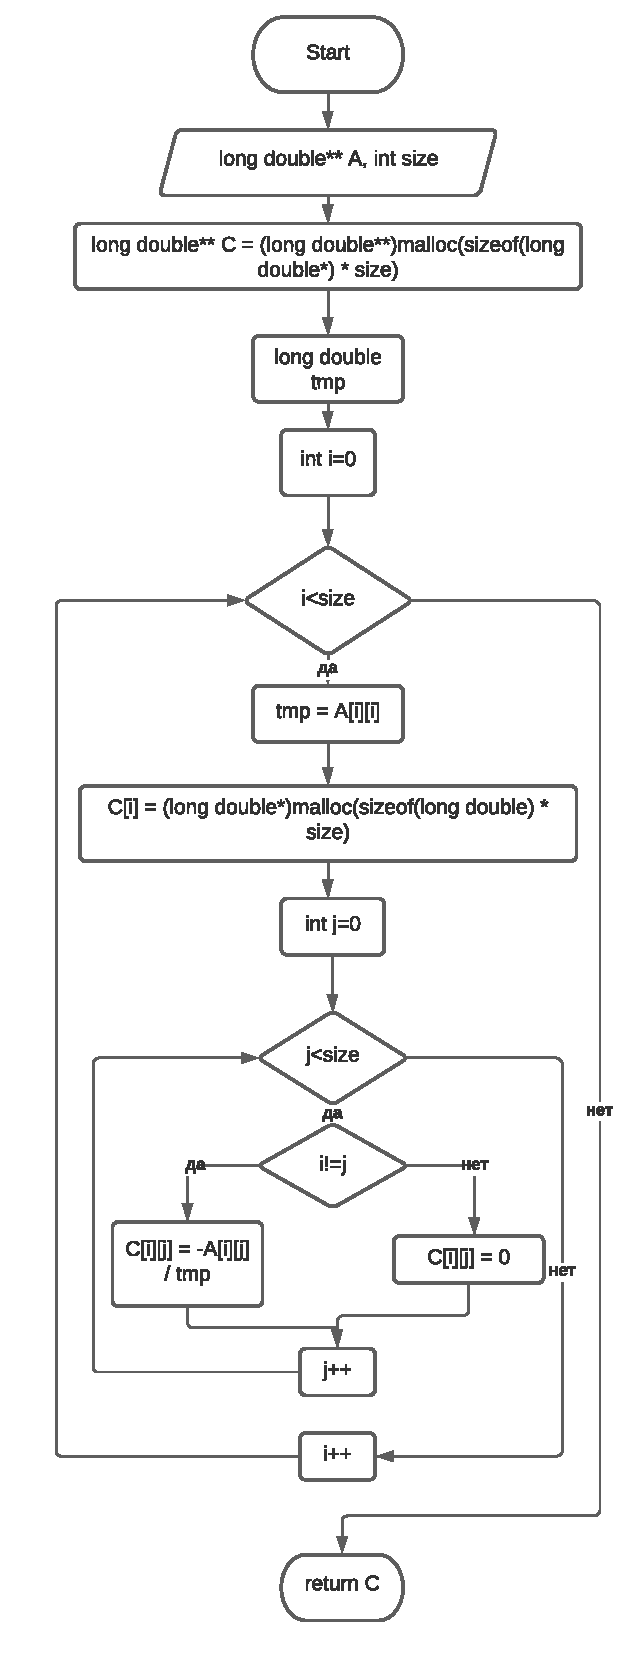
\includegraphics[scale=0.5]{block3.pdf}

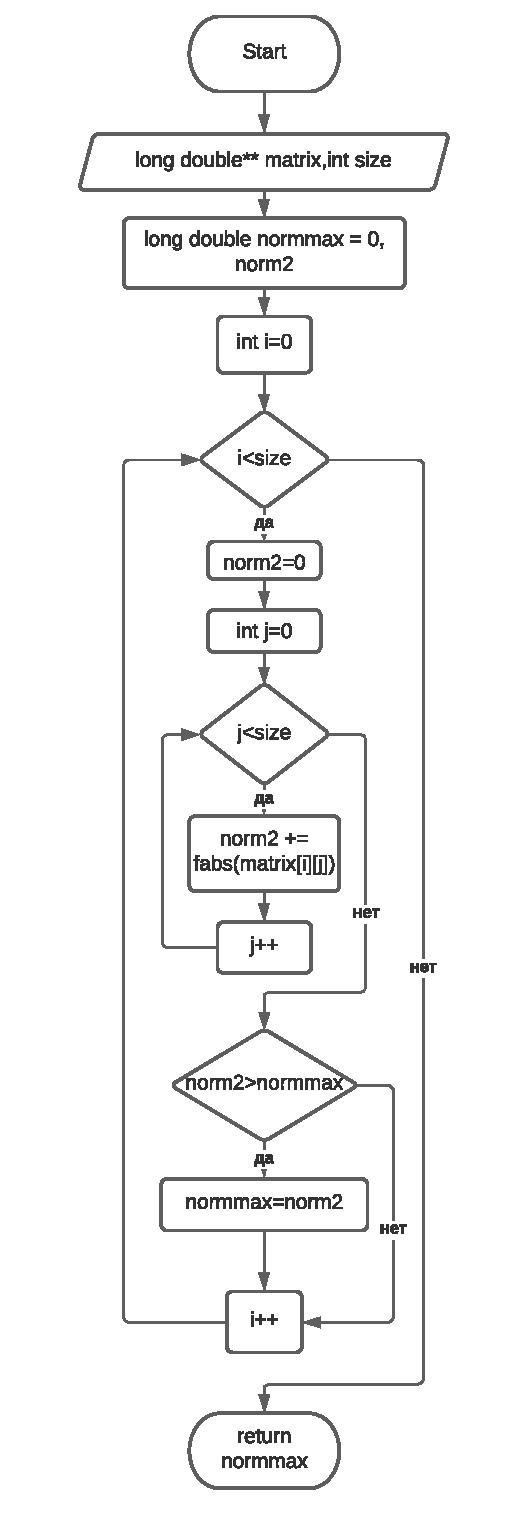
\includegraphics[scale=0.5]{block4.pdf}

Функция long double* ColumnRead(FILE* file, int size)

\includegraphics[scale=0.5]{block2.pdf}

\section{Численный анализ решения задачи}

\subsection{Зависимость относительной погрешности от числа обусловленности}

\includegraphics[scale=0.5]{1.pdf}

На данном графике видно, что с ростом числа обусловленности от 10 до 50000 относительная погрешность вычислений (разница точного решения и численного, деленная на точное решение) возрастает почти линейно. 

\subsection{Зависимость относительной погрешности решения от относительной погрешности возмущения}

\includegraphics[scale=0.5]{2.pdf}

Относительная погрешность решения при большем числе обусловленности больше, чем при меньшем числе обусловленности.


\section{Краткие выводы}

Была решена задача нахождения решения СЛАУ методом вращений.

Были выявлены зависимости относительной погрешности решения от числа обусловленности и относительной погрешности решения от относительной погрешности возмущения столбца свободных членов.


\end{document}
